\chapter{Execution-based evaluation, correction gates, and release tests}
\label{ch04-execution-correction-gates-release-tests}
Mehta (\href{https://arxiv.org/abs/2603.25764}{2026}) analyzed 1,750 coding-agent trajectories across 50 tasks and four models and found a sharp divide between submission and correctness. One model submitted an answer in every trial, yet an external oracle found that it resolved only 44 percent of the tasks. Its semantic failures were often silent, confident, and consistent across repeated runs. Most models also modified code that was already correct.

The study provides directional evidence rather than a general estimate of coding-agent failure rates. It covers one author's analysis, a limited task set, and four models, without a controlled design for estimating prevalence across agents or workloads.

\begin{figure}[htbp]
\centering
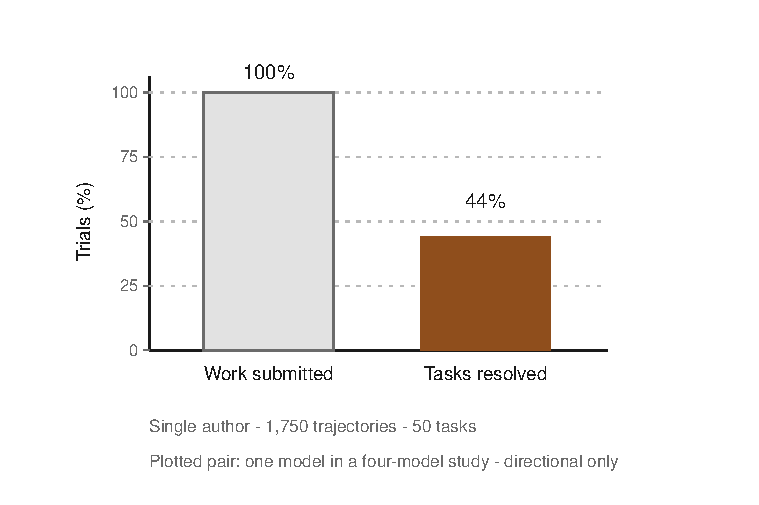
\includegraphics{figures/ch04-submission-resolution.pdf}
\caption{Across 1,750 trajectories covering 50 tasks and four models, one model submitted work in 100\% of its trials but resolved only 44\% under an external oracle.}
\end{figure}

Submission, consistency, and self-assessment are all produced by the process under evaluation. A model can repeatedly generate the same incorrect patch, describe it with stable confidence, and end each run cleanly. Those signals characterize the trajectory, but they do not show that the repository moved from a failing state to a working one. Acceptance therefore requires evidence of an observable state transition, verified by a system outside the inference process that proposed the change.

The evidence base for this chapter is thin. The actions below therefore ask readers to execute and measure work on their own systems rather than adopt a reported threshold. Six evidence items support the three practices developed here. Five are source syntheses, and one is a controlled experiment. One entry has no strong supporting evidence item.

The practical unit is a gate that can stop candidate work from propagating. The candidate runs under explicit constraints, any correction attempt receives the evidence produced by verification, and a compact set of representative tasks is replayed whenever the system changes.

Four adjacent controls appear in the companion catalog rather than in this chapter. For an agent that submits on nearly every trial, score verified resolution separately from submission and include tasks that test whether it can abstain. For a tool that can fail while returning a plausible success string, detect silent tool errors explicitly. For a loop that can retry indefinitely, impose a turn budget. When per-candidate verification cost determines how often a gate can run, include that cost in the system's accounting.

\hypertarget{make-execution-decide-whether-work-moves}{%
\section{Make execution decide whether work moves}\label{make-execution-decide-whether-work-moves}}

Two directional synthesis items support execution-gated evaluation, but neither is a controlled estimate of its effect. AgentForge, from Kumar et al.~(\href{https://arxiv.org/abs/2604.13120}{2026}), describes an evaluator that runs candidate work in resource-bounded, network-isolated sandboxes and permits propagation only after successful execution. SWE-bench, from Jimenez et al.~(\href{https://arxiv.org/abs/2310.06770}{2023}), establishes executable repository repair as an evaluation form.

The AgentForge preprint is unrefereed, evaluates a single configuration, and reports one sample from each agent. Its headline result also conflicts with the published range for that configuration and has not been independently replicated, so I omit the number. These limits prevent either source from establishing a general failure rate or a measured advantage for execution gating. They do not weaken the mechanism worth testing: run the artifact in a constrained environment, and let the observed result determine whether it can proceed.

A plausible patch is only text until the repository accepts it. It may fail to compile, violate a type constraint, pass a visible test while failing the broader suite, produce the wrong output, or depend on undeclared state left in the workspace. Reading the patch can reveal some of these defects. Executing it produces evidence from the system the change is supposed to affect.

This changes the acceptance question. A confidence score asks the process that produced an answer to characterize its own answer. An execution check asks a compiler, test runner, package builder, schema validator, or deployment probe whether a specified transition occurred.

Park and Choi (\href{https://arxiv.org/abs/2607.25152}{2026}) held an agent and its tool surface fixed while changing the evaluator's information channel. Across 54 cycles, the agent claimed improvement every time, although 56 percent of measured deltas were zero or negative; the self-verdict gate accepted every cycle and eroded the best reached state by 19 percent. On a boundary task whose success was verifiable from the artifact, the same judge's gap disappeared. This is strong evidence within the preregistered testbed that a gate must observe the state in which success is defined.

The result is an oracle only for the behavior the check observes. A passing unit test does not establish safe deployment, and a successful build does not establish semantic correctness. Its evidentiary value comes from being produced causally downstream of the candidate artifact rather than by the process that proposed it.

\Needspace{5\baselineskip}

The architecture has three owners:

\begin{itemize}
\tightlist
\item
  The agent owns the proposed change.
\item
  A sandbox controller owns the execution environment and the authority to start a run.
\item
  A release controller owns downstream state and changes it only after the sandbox returns an admissible result.
\end{itemize}

Separating these roles prevents the producer from turning a claim of success into release state by writing a status field, omitting failed checks, or selecting which results to report.

A sandbox needs enough isolation for its verdict to be interpretable. Each run should begin from a known repository snapshot and receive only the inputs permitted by the task. Bound wall-clock time, CPU, memory, process count, and disk use. Deny network access unless the task explicitly requires a named endpoint. Capture standard output, standard error, exit status, resource termination, and declared artifacts, then dispose of the environment after the verdict.

Reusing a mutable workspace is cheaper, but it allows one attempt to seed the next through generated files, caches, installed dependencies, or surviving processes. The later result then reflects both the current candidate and undeclared state inherited from earlier attempts.

Network isolation serves measurement as well as security. An unrestricted candidate can fetch an undeclared dependency, consult a changing service, upload material, or pass because a remote cache happens to contain the required state. When a task genuinely depends on a network service, expose a controlled substitute or record the service version and responses. Otherwise identical artifacts can receive different verdicts for reasons unrelated to their behavior.

Resource bounds make nontermination an explicit outcome. A process killed after exceeding a declared limit should be recorded separately from a failed assertion or an ordinary completion. The gate should identify which bound fired. Parallel tests may exhaust memory, while a surviving child process may trigger the process-count or wall-clock limit.

The acceptance contract should be readable without inspecting the controller:

\begin{verbatim}
command:       verify-change
expected:      exit status 0
required:      reports/test-results.json
               build/package.tar.gz
artifact rule: each required file exists and is non-empty
timeout:       12 minutes
network:       denied
\end{verbatim}

The task definition fixes the command before the candidate encounters a failure. The expected condition names something more specific than ``works correctly.'' The artifact rules remove another common ambiguity: a wrapper can exit successfully after skipping the operation that should have produced the evidence.

Exit status alone is often too weak. A test runner can return zero after discovering no tests. A report generator can create an empty file. A shell pipeline can discard the failure status of an earlier command. A zero exit status shows that the final process ended successfully, not necessarily that the intended work occurred.

The controller should therefore validate the structure on which the verdict depends. Depending on the task, that may mean checking for an expected test count, a parseable result file, a package containing required members, or a deployment probe tied to the candidate version. These are mechanical checks. They do not require the controller to infer the patch's semantics.

Environment failure must remain distinct from candidate failure. If the sandbox image cannot be pulled, the verifier is absent, or the runner loses its workspace, marking the candidate incorrect corrupts the evaluation. Allowing it to pass because verification could not start corrupts release state. The correct outcome is an infrastructure error that blocks propagation and may be retried without crediting or blaming the candidate.

Infrastructure errors should still be counted. A run set repeatedly thinned by environment failures no longer represents the intended sample of attempts, even when those failures are excluded from candidate scores.

State should move monotonically through the gate. A candidate begins unverified, receives an immutable run record, and becomes eligible for the next stage only when that record satisfies the contract. Any modification creates a new candidate identity and invalidates the earlier verdict. When a verdict is keyed only to a branch name or task identifier, changed bytes can inherit evidence produced for different work.

In my own agent-workflow system, I reject any acceptance criterion that says only that a result ``works correctly.'' The rejection occurs during decomposition, before work begins. Each criterion must name a command and an exit condition. At the end of every turn, a lifecycle check also verifies that declared output files exist and contain data.

That lifecycle check runs deterministically, but a model evaluates the filesystem and provides only advisory judgment. Enforced refusal requires a command hook whose nonzero exit ends the turn. The example shows how a gate can begin in the task contract, but it does not provide evidence for the general claim.

My repository-scale benchmark suite uses a deterministic verifier as the primary scorer for every task. Additional judgment layers can flag suspicious trajectories, but they cannot replace or override the execution verdict. This preserves one stable state transition even when the optional analysis changes.

Execution is not suitable for every task. Architecture proposals, interface critiques, threat models, and underspecified behavioral changes may have no executable oracle. Those tasks require a separate, calibrated judgment lane, which Chapter 5 develops.

Executable checks also have a coverage boundary. They can establish that a candidate compiled, passed a selected suite, produced required artifacts, and stayed within its resource envelope. They cannot establish that untested inputs, longer operating periods, or a different production topology will behave the same way.

Record only the narrowest downstream claim justified by the run: test-eligible, build-eligible, or deployment-eligible.

The run record also provides the evidence needed for correction. A failed command, assertion diff, resource termination, or missing artifact gives the next attempt information that was unavailable when the candidate was produced. Without new evidence, another model pass is repetition presented as diagnosis.

\hypertarget{let-failed-runs-change-the-next-attempt}{%
\section{Let failed runs change the next attempt}\label{let-failed-runs-change-the-next-attempt}}

A retry that begins with the same prompt, evidence, and workspace state has learned nothing about the failure. Sampling may produce a different answer, but it does not direct the model toward the error. The next pass may repeat the faulty premise, replace a correct intermediate step, or elaborate the same mistaken conclusion. Calling that pass ``reflection'' does not add information.

Huang et al.~(\href{https://arxiv.org/abs/2310.01798}{2023}) evaluated intrinsic self-correction on reasoning tasks using 2023-era models. Self-correction often failed and sometimes reduced performance, while reliable external feedback improved it. This is strong evidence for the systems studied, not an estimate of every current coding system. Newer models may change the magnitude of the effect.

The operational default should therefore be asymmetric: authorize another attempt when an external observation changes the available evidence, not merely because the previous attempt failed.

An external observation originates outside the inference that produced the candidate. Examples include a test assertion, compiler diagnostic, tool response, verifier verdict, or deployment probe. A critique produced by another model call does not become external evidence merely because it was generated separately. Without access to an independent observation, it remains another inference over substantially the same record.

The distinction is informational. Suppose an agent changes a parser because it concludes that empty fields should be discarded. Re-reading the issue may reinforce that interpretation. A failing test showing that an empty field must preserve its position introduces a counterexample. The next attempt can now revise a specific assumption rather than search an unconstrained space of possible mistakes.

This closes the loop opened by the sandbox:

\begin{verbatim}
candidate
    -> sandbox run
        -> pass: eligible for downstream gate
        -> fail: immutable result returned to correction step
            -> revised candidate
                -> new sandbox run
\end{verbatim}

The correction step does not modify the verdict. It consumes the failed candidate and its run record, then emits a new candidate with a new identity. This preserves the history needed to distinguish recovery from repeated failure. It also prevents revised bytes from inheriting a passing result produced by an earlier version.

\Needspace{5\baselineskip}

Feedback should contain enough detail to distinguish the failed path without flooding the next attempt with unrelated output. A useful package identifies:

\begin{itemize}
\tightlist
\item
  the command that ran;
\item
  the candidate version;
\item
  the exit status;
\item
  the failed check and relevant diagnostic;
\item
  any resource limit or termination that fired; and
\item
  a pointer to the complete run record.
\end{itemize}

When a report is large, retain the full output as an artifact and present a mechanically selected excerpt. The complete evidence remains available when the excerpt omits the decisive line.

Selection should remain mechanical wherever possible. When one model decides which failures another model sees, it may omit evidence that contradicts its diagnosis or overemphasize a familiar error. Test frameworks already expose failed case names, assertion differences, stack traces, and structured result records. Use those fields before asking another inference to summarize them.

The deployed system must also have access to the feedback channel. Chapter 2 required a retry baseline to use only failure signals available in deployment. Otherwise the experimental retry arm receives information that the product will not have. Here that requirement becomes concrete: a retry is externally informed only when its signal comes from a tool or observation that the deployed loop can obtain at that point in its lifecycle.

This prevents a subtle comparison error. An evaluator might show the retry arm the hidden reference test that rejected a patch, while the production agent sees only public tests. The experiment then measures correction under privileged supervision, not the deployed retry policy. Hidden checks may still determine the final score, but their diagnostics should enter the correction loop only when production has an equivalent feedback channel.

External observations also have authority boundaries. A unit-test failure can justify another code attempt. A package-registry outage says little about the candidate and belongs in infrastructure handling. A deployment probe run against the wrong version may direct the model to repair code that was never exercised. Before authorizing another attempt, the controller must classify the observation as a candidate failure, an environment failure, or an evaluator failure.

Reliable feedback may still be incomplete. A failing test can expose a symptom without identifying its cause. A compiler diagnostic may point to a generated file even though the defect originated in source configuration. The next attempt should use the observation to constrain its diagnosis before modifying the artifact. Execution adds information to the correction loop, but the observation does not necessarily contain the remedy.

Faulty feedback creates a directed failure mode. An incorrect expected value, nondeterministic test, stale fixture, or verifier attached to the wrong artifact can push successive revisions farther from correct behavior. The loop may then appear to converge while following a bad oracle. Preserve the raw run records and candidate lineage so an operator can determine whether each correction followed valid evidence.

\Needspace{5\baselineskip}

Retry limits remain necessary even when every attempt receives a genuine new signal. A sequence of distinct failing tests can consume an unbounded budget, and each revision can create a new failure surface. Stop conditions should distinguish:

\begin{itemize}
\tightlist
\item
  a fixed attempt limit;
\item
  repeated identical failures;
\item
  infrastructure failures; and
\item
  exhaustion of the gate's resource budget.
\end{itemize}

A new observation may justify another attempt, but it does not justify unlimited attempts.

Correction belongs to the evaluation architecture, not to a personality attributed to the model. The model proposes revisions. The surrounding system determines whether the evidence changed, whether another attempt may run, and whether the resulting artifact may propagate. That division continues to hold when the model, prompt, or language of correction changes.

\hypertarget{turn-repeated-trials-into-a-release-test}{%
\section{Turn repeated trials into a release test}\label{turn-repeated-trials-into-a-release-test}}

Support for the repeated-trial metric comes from one source. tau-bench, from Yao et al.~(\href{https://arxiv.org/abs/2406.12045}{2024}), evaluates interactive, multi-turn tool use with executable oracles across repeated trials and introduces \(\mathrm{pass}^{k}\) as a reliability measure.

The paper does not evaluate two parts of the practice recommended here: selecting a team's own tasks and replaying them for every release. Those are transfers from benchmark design into release engineering. The measured result supports repeated trials under executable evaluation, not the claim that a particular local task set or release policy will predict production reliability.

The transfer begins with the workload set established at the end of Chapter 3. The golden set is a compact collection of completed tasks whose initial repository states can be reconstructed and whose outcomes have unambiguous executable checks. Each versioned case should keep together:

the original request;
the starting repository state;
the allowed tools and turn constraints;
the sandbox contract; and
the verifier.

A merged patch may help reconstruct the expected behavior, but it should not appear in the agent's context.

Real tasks preserve local constraints that public benchmarks cannot know. A repository may require generated files to remain synchronized, prohibit a dependency, enforce a custom migration check, or treat a particular warning as release-blocking. Those details determine whether work is acceptable in that repository. A general coding score does not encode them.

The set should remain small enough to run repeatedly and inspect when it changes. Its purpose is to discriminate between releases on a controlled sample, not to approximate every production request. Each case should represent at least one of three things: a failure that would be costly if it returned, a workflow the system performs frequently, or an interaction whose state cannot be inferred from a static answer. Ten nearly identical formatting fixes provide less coverage than a smaller set spanning localization, modification, testing, tool failure, and recovery.

Interactive cases belong in the set when the deployed system uses tools across turns. A final patch alone does not show whether the agent opened the right file, preserved state after a failed command, recovered from a tool error, or incorporated a later observation into an earlier plan. Replaying the trajectory under the deployed tool and turn constraints exposes sequencing and recovery failures that final-answer scoring cannot observe.

Each case needs a stable identity and immutable versions. Changing the request, starting repository, tool contract, sandbox policy, or verifier creates a different case and should produce a new version. Rewriting an existing case beneath prior scores can manufacture apparent improvement by removing a difficult condition or exposing more of the solution.

Run each case more than once for the same release candidate. The repeated-trial statistics from Chapter 1 govern the experimental design and do not need to be rebuilt here. For release control, \(\mathrm{pass}^{k}\) asks whether all \(k\) of \(k\) trials passed. One failed trajectory breaks the sequence.

The result describes a single release candidate only when its configuration remains pinned across the sequence. Chapter 1's apparatus record applies to every trial, including the model version and decoding settings. Pinning does not guarantee independence. Shared caches, mutable services, provider incidents, and reused infrastructure can correlate outcomes, which limits the analyses the sequence supports.

\(\mathrm{pass}^{k}\) reflects a different operational question from \(\mathrm{pass}@k\):

\begin{verbatim}
same k trials
    |
    +-> all-k reliability
    |     all k of k trials passed
    |     one failed trajectory breaks the sequence
    |
    +-> at-least-one success
          at least one trajectory succeeded
          several attempts were available

choose the metric whose failure semantics resemble deployment

workflow must complete reliably without supervision
    -> stronger reason to use all-k reliability
\end{verbatim}

\(\mathrm{pass}@k\) asks whether at least one acceptable trajectory can be found when several attempts are available. \(\mathrm{pass}^{k}\) asks whether every trajectory in a required sequence succeeds. Neither is universally correct. A supervised workflow that can select among alternatives may justify \(\mathrm{pass}@k\). A workflow expected to complete reliably without intervention has a stronger reason to use \(\mathrm{pass}^{k}\).

The value of k comes from release policy, not from the benchmark. Increasing k makes intermittent failures easier to observe and the gate harder to satisfy. It also increases cost and gives evaluator noise more opportunities to block promotion. Choose k based on the consequence of one failed production run, the variance observed during pilot repeats, and the budget available for evaluating each release candidate.

The number of cases interacts with that decision. Under a strict all-trials rule, the chance that at least one verdict fails because of evaluator noise grows with both the set size and k. This is the multiplicity problem that Chapter 1 assigns to claims spanning many tasks. A larger gate therefore requires either a very low per-run evaluator error rate or an explicit policy defining how many case failures block promotion.

The comparison unit is the fully specified system release. Record the model identifier, prompt version, tool definitions, orchestration code, sandbox image, task-set version, retry policy, and verifier version. Any of these components can change the trajectory distribution. A result labeled only with a model name erases much of what teams actually change between releases.

The release record can remain mechanically small:

\begin{verbatim}
release:         candidate-2026-07-28
system_digest:   6f5c...
task_set:        golden-07
repeats:         k
baseline:        production-previous
case_verdicts:   stored run records
promotion_rule:  recorded before execution
\end{verbatim}

The digest binds the verdict to the evaluated configuration. The case verdicts link to the sandbox evidence. The promotion rule is recorded before the comparison begins. Otherwise the same regression can be accepted for a favored release and rejected for another.

Compare the candidate with a stored baseline using the same case versions and execution policy. Report both per-case outcomes and run-to-run spread alongside the aggregate release verdict. An aggregate value can conceal a complete regression on one critical workflow behind stable performance elsewhere. A case-only view can be dominated by one noisy verifier. Both levels are needed to locate the change and determine whether the promotion rule was met.

Because the candidate and baseline run the same cases, their outcomes are paired by construction. Chapter 1's paired analysis applies. Treating the releases as independent samples discards a dependency that the design already provides.

The baseline must remain executable. A table copied from an earlier report is not enough. Sandbox images disappear, dependencies move, and tool services change behavior. Re-running at least a sample from the stored baseline helps separate candidate drift from evaluator drift. When the old release also fails under the current infrastructure, the comparison has lost its fixed reference and promotion should block until the cause is understood.

My search-visibility measurement project treats a model update as a deployment. It replays a fixed prompt corpus against a stored model-version baseline and combines a statistical comparison with an absolute change threshold, producing pass, warning, or failure exit states for continuous integration. The controls answer different questions. Statistical comparison reduces the chance that sampling noise decides promotion. The absolute threshold prevents a detectable but operationally trivial change from doing so. This example supplies no evidence for either threshold.

CodeProbe (\href{https://github.com/sjarmak/codeprobe}{public repository}) uses a different gate. It blocks a release tag unless the two most recent full-mode acceptance verdicts both pass. Those verdicts come from successive acceptance-loop iterations, not repeated trials of one pinned candidate. The rule is therefore a check over acceptance history, not a \(\mathrm{pass}^{k}\) measurement. Its requirement of two consecutive passes is local to that system and should not be treated as a recommended value of \(k\).

Golden sets decay even when their files remain unchanged. Production work moves to new frameworks, repositories acquire new checks, tool interfaces change, and models may become adapted to repeatedly exposed cases. A set that once represented costly failures can gradually become a test of a narrow historical workflow. Treat the set as production test data, with named ownership, review, and retirement criteria.

Maintenance should preserve longitudinal meaning. Add a case when a production failure reveals a missing class of behavior. Do not silently replace the old set, because the new score will no longer be comparable with earlier releases. When feasible, run an overlap period, report performance on the shared cases, and establish a new baseline for the revised set. Retire a case when its workload no longer exists or its oracle no longer represents the current contract.

Public benchmarks can inform case design and reveal task forms worth reproducing locally.

SWE-bench provides directional support for executable repository repair. MultiAgentBench, from Zhu (\href{https://arxiv.org/abs/2503.01935}{2025}), does the same for broader interaction-centered evaluation. Their architectural contribution is to place an environment, tools, state, and an outcome check inside the evaluated unit rather than scoring final-answer text alone.

Neither benchmark measures the effect of selecting a team's own tasks or replaying them for each release. Nor does either estimate the gap between public benchmark performance and reliability in a particular repository, tool policy, or release process. No evidence item supporting this entry supplies a conversion factor.

The local release test answers a narrower question: did this fully specified system preserve acceptable behavior on a controlled sample of local work?

Once the set participates in release, a failure should trigger diagnosis before any threshold is revised. Determine whether the candidate changed, the case changed, or the evaluator changed. Route valid candidate failures through the external-feedback correction loop, then rerun the entire required sequence for the revised candidate. Reusing passing trials from before a modification would attach evidence to a system that no longer exists.

\hypertarget{build-the-first-gate}{%
\section{Build the first gate}\label{build-the-first-gate}}

Begin with five to ten tasks drawn from merged work rather than from a generic capability suite. Choose tasks whose starting states can be reconstructed and whose acceptable outcomes can be verified without interpretive judgment. The first set can remain small because its purpose is to establish a release path that produces trustworthy evidence. Expand it when production failures reveal behaviors the initial sample did not cover.

Wrap each task in a sandboxed run. Define the command the controller will execute, the exit condition it will accept, and the artifacts that must exist afterward. Bound resource use, isolate the network, and preserve the complete run record.

Run the current production system through the same cases and evaluator before testing a candidate release. Its observed performance becomes the baseline. This replaces remembered claims, old summary tables, or results produced under a different environment.

When a candidate fails, return the raw evidence to the correction loop together with the candidate identity. Do not authorize a revision that has learned nothing beyond the original request. Every modified candidate receives a new identity, starts in a clean sandbox, and earns a new verdict. Infrastructure failures remain blocking, but they do not count as candidate failures.

Replay the set whenever the model, prompt, tools, orchestration, sandbox, or verifier changes. Measure \(\mathrm{pass}^{k}\) across the chosen repeats, retain the per-case outcomes and run-to-run spread, and compare the candidate with the executable baseline.

Record the promotion rule before running the first candidate comparison. When experience shows that the gate is too strict or too permissive, change the policy as a versioned decision and establish a new baseline where necessary. Adjusting the threshold after seeing a result turns the rule into an explanation for a decision already made.

Keep tasks without executable checks in a separate lane. They are not lesser tasks, but forcing them through weak proxies would make the gate appear more complete than it is. Chapter 5 develops the calibrated judgment process those tasks require.

\section*{Sources and evidence}

\textbf{Motivating observation and companion entry}

\begin{itemize}
\tightlist
\item
  Directional evidence: Mehta, A. (2026). Confident and Wrong: Silent Semantic Failures in Coding Agents. arXiv:2603.25764. Analysis of 1,750 trajectories across 50 tasks and four models; single-author, limited-sample observational finding. Supports the companion-only entry on scoring verified resolution separately from submission.
\end{itemize}

\textbf{\texttt{ground-evaluation-in-execution}}

\begin{itemize}
\tightlist
\item
  Directional evidence: AgentForge (Kumar et al.~2026, arXiv:2604.13120). Execution-grounded evaluation in resource-bounded, network-isolated sandboxes, with propagation gated on execution results. Unrefereed preprint; single configuration; one sample per agent.
\item
  Directional evidence: SWE-bench (arXiv:2310.06770), from Jimenez et al.~2023. No figure carried.
\item
  Strong evidence for externally grounded gating in the measured testbed: Park, H., and Choi, B. (2026), ``When Do Agent Loops Mistake Stagnation for Progress?'' arXiv:2607.25152. The 54-cycle result does not estimate a general agent failure rate.
\end{itemize}

\textbf{\texttt{gate-self-correction-on-external-feedback}}

\begin{itemize}
\tightlist
\item
  Strong evidence: Huang, J., et al.~(2023). Large Language Models Cannot Self-Correct Reasoning Yet. ICLR 2024. arXiv:2310.01798.
\end{itemize}

\textbf{\texttt{golden-set-pass-k}}

\begin{itemize}
\tightlist
\item
  Strong evidence: tau-bench (Yao, Shinn, Razavi \& Narasimhan 2024, arXiv:2406.12045). Introduces and measures \(\mathrm{pass}^{k}\) on interactive, multi-turn tool-use tasks with executable oracles. Using a team's own tasks and replaying the set per release are transfers beyond the measured findings.
\item
  Directional evidence: SWE-bench (arXiv:2310.06770).
\item
  Directional evidence: MultiAgentBench (Zhu 2025, arXiv:2503.01935).
\end{itemize}

\textbf{Author-system illustration cited inline}

\begin{itemize}
\tightlist
\item
  Not an evidence item: CodeProbe, the author's task-mining evaluation tool, \href{https://github.com/sjarmak/codeprobe}{public repository}. Named inline for the consecutive-release acceptance gate described above, which is narrative illustration.
\end{itemize}
